\documentclass[aspectratio=169,11pt]{beamer}
\usetheme{Madrid}
\usecolortheme{default}
\setbeamertemplate{navigation symbols}{}
\usepackage[utf8]{inputenc}
\usepackage[T1]{fontenc}
\usepackage{lmodern}
\usepackage[indonesian]{babel}
\usepackage{graphicx}
\usepackage{booktabs}
\usepackage{array}
\usepackage{tikz}
\usetikzlibrary{arrows.meta,positioning,shapes.geometric,calc,decorations.pathreplacing}
\usepackage{listings}
\usepackage{xcolor}
\usepackage{ragged2e}
\usepackage{adjustbox}
\usepackage{hyperref}
\usepackage{amsmath}
\usepackage{amsfonts}
\usepackage{multicol}

\graphicspath{{assets/}{../M01/assets/}{../M02/assets/}}

\definecolor{DeepNavy}{HTML}{0B1220}
\definecolor{Navy}{HTML}{12355B}
\definecolor{Blue}{HTML}{1F77B4}
\definecolor{Teal}{HTML}{00A6A6}
\definecolor{Gold}{HTML}{F2B705}
\definecolor{LightBlue}{HTML}{EAF4FF}
\definecolor{LightTeal}{HTML}{E7FAF8}
\definecolor{SoftGray}{HTML}{F4F6F8}
\definecolor{CodeBg}{HTML}{F8FAFC}
\definecolor{DarkText}{HTML}{15202B}
\definecolor{Purple}{HTML}{6F42C1}
\definecolor{SoftRed}{HTML}{FDECEC}
\definecolor{SoftGreen}{HTML}{EAF7EA}

\setbeamercolor{title}{fg=white}
\setbeamercolor{frametitle}{fg=white,bg=Navy}
\setbeamercolor{structure}{fg=Blue}
\setbeamercolor{normal text}{fg=DarkText,bg=white}
\setbeamercolor{block title}{fg=white,bg=Navy}
\setbeamercolor{block body}{fg=DarkText,bg=LightBlue}
\setbeamercolor{alerted text}{fg=Gold}
\setbeamerfont{title}{size=\LARGE,series=\bfseries}
\setbeamerfont{subtitle}{size=\large}
\setbeamerfont{frametitle}{size=\large,series=\bfseries}
\setbeamerfont{footline}{size=\fontsize{7.2}{8}\selectfont}
\setbeamertemplate{itemize items}[circle]

\lstdefinestyle{py}{
  language=Python,
  basicstyle=\ttfamily\scriptsize,
  keywordstyle=\color{Blue}\bfseries,
  commentstyle=\color{Teal},
  stringstyle=\color{Gold!70!black},
  showstringspaces=false,
  breaklines=true,
  frame=single,
  rulecolor=\color{Navy!35},
  backgroundcolor=\color{CodeBg},
  tabsize=4,
  columns=fullflexible
}
\lstset{style=py}

\tikzset{
  box/.style={rounded corners=3pt, draw=Navy!70, fill=LightBlue, thick, minimum height=8mm, inner sep=2.2mm, align=center},
  greenbox/.style={rounded corners=3pt, draw=Teal!70!black, fill=LightTeal, thick, minimum height=8mm, inner sep=2.2mm, align=center},
  redbox/.style={rounded corners=3pt, draw=red!50!black, fill=SoftRed, thick, minimum height=8mm, inner sep=2.2mm, align=center},
  darkbox/.style={rounded corners=3pt, draw=Navy, fill=Navy, text=white, thick, minimum height=8mm, inner sep=2.2mm, align=center},
  arr/.style={-{Latex[length=2.3mm]}, thick, draw=DarkText}
}

\newcommand{\mkfooter}{Pemrograman untuk Ilmu Data dan Komputasi}
\newcommand{\prodi}{Program Studi Matematika ITERA}
\setbeamertemplate{footline}{%
\leavevmode%
\hbox{%
\begin{beamercolorbox}[wd=.45\paperwidth,ht=2.35ex,dp=.95ex,leftskip=1.0ex]{author in head/foot}\mkfooter\end{beamercolorbox}%
\begin{beamercolorbox}[wd=.37\paperwidth,ht=2.35ex,dp=.95ex,center]{author in head/foot}\prodi\end{beamercolorbox}%
\begin{beamercolorbox}[wd=.18\paperwidth,ht=2.35ex,dp=.95ex,rightskip=1.0ex plus1fil]{author in head/foot}\hfill\insertframenumber/\inserttotalframenumber\end{beamercolorbox}%
}%
}

\title[\mkfooter]{Pertemuan 5: Kompleksitas Algoritma dan Big-O}
\subtitle{Menghitung kerja program dari potongan kode}
\author{Rifky Fauzi dan Triyana Muliawati, S.Si., M.Si.}
\institute{Program Studi Matematika, Institut Teknologi Sumatera}
\date{Ganjil 2026/2027}

\begin{document}

% 1
\begin{frame}[plain]
\begin{tikzpicture}[remember picture,overlay]
\IfFileExists{assets/tech_bg.png}{%
\node[anchor=center] at (current page.center){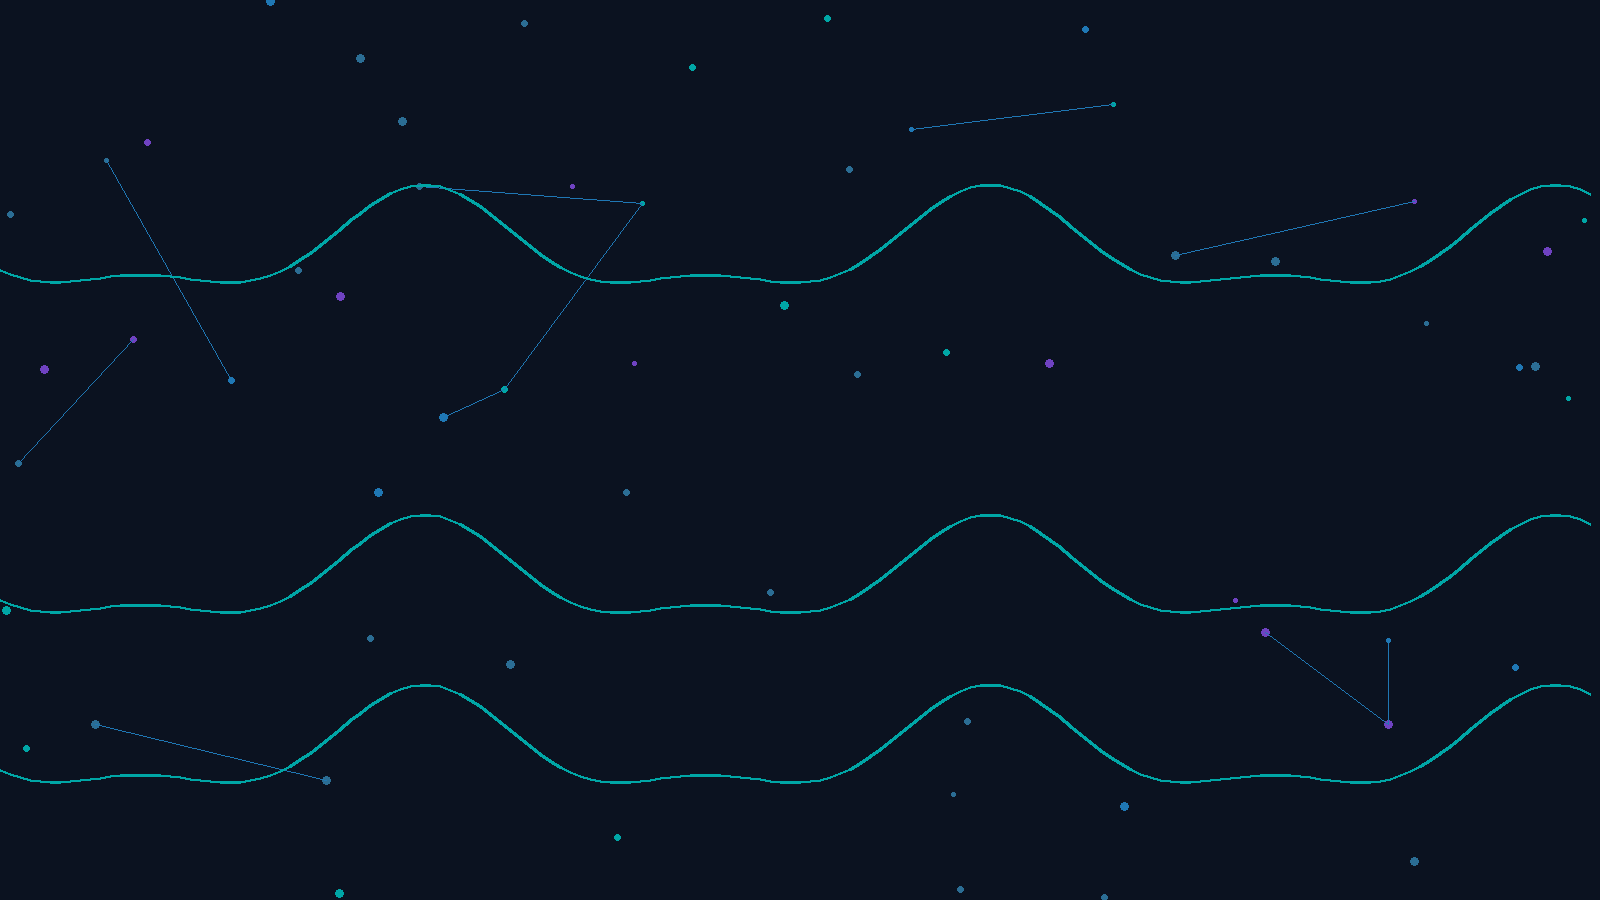
\includegraphics[width=\paperwidth,height=\paperheight]{assets/tech_bg.png}};%
}{\IfFileExists{../M01/assets/tech_bg.png}{%
\node[anchor=center] at (current page.center){
\includegraphics[width=\paperwidth,height=\paperheight]{../M01/assets/tech_bg.png}};%
}{%
\fill[DeepNavy] (current page.south west) rectangle (current page.north east);
\fill[Blue!20,opacity=.18] ([xshift=1.2cm,yshift=-1.2cm]current page.north west) circle (3.2cm);
\fill[Teal!30,opacity=.16] ([xshift=-1.2cm,yshift=1cm]current page.south east) circle (3.8cm);%
}}
\fill[DeepNavy,opacity=.84] (current page.south west) rectangle ([xshift=8.15cm]current page.north west);
\node[anchor=north west,text=white,align=left,text width=6.65cm] at ([xshift=.65cm,yshift=-.55cm]current page.north west){%
{\hyphenpenalty=10000\exhyphenpenalty=10000\fontsize{20}{22.5}\selectfont\bfseries Pertemuan 5\\Kompleksitas Algoritma\\dan Big-O}\\[3mm]
{\fontsize{14.5}{17}\selectfont Pemrograman untuk Ilmu Data\\dan Komputasi}\\[2.5mm]
{\fontsize{10.5}{12}\selectfont MA25-21008 \quad Kelas RA dan RB}\\[5mm]
{\fontsize{10}{11.5}\selectfont Rifky Fauzi\\Triyana Muliawati, S.Si., M.Si.}\\[3mm]
{\fontsize{9.3}{10.8}\selectfont Program Studi Matematika\\Institut Teknologi Sumatera\\Semester Ganjil 2026/2027}
};
\node[anchor=north east,fill=white,fill opacity=.95,text opacity=1,rounded corners=3pt,inner sep=4.2mm,text width=6.95cm] at ([xshift=-.35cm,yshift=-.78cm]current page.north east){%
{\fontsize{13}{15}\selectfont\bfseries Alur pertemuan}\\[2mm]
\begin{itemize}\small
  \item Dari terminasi ke jumlah langkah.
  \item Menurunkan $T(n)$ dari kode.
  \item Mengambil orde dominan: Big-O.
  \item Membandingkan beberapa algoritma anagram.
  \item Membaca biaya operasi list melalui eksperimen.
\end{itemize}
};
\end{tikzpicture}
\end{frame}

% 2
\begin{frame}[fragile]{Dari M4: program berhenti, lalu berapa kerjanya?}
\begin{columns}[T]
\column{.49\textwidth}
\begin{block}{Pertanyaan M4}
Program ini berhenti atau tidak?
\end{block}
\begin{lstlisting}
i = n
while i > 0:
    i = i // 2
\end{lstlisting}
\column{.49\textwidth}
\begin{block}{Pertanyaan M5}
Jika berhenti, berapa banyak langkah yang kira-kira dilakukan saat $n$ membesar?
\end{block}
\begin{lstlisting}
test = 0
for i in range(n):
    for j in range(n):
        test = test + i*j
\end{lstlisting}
\end{columns}
\vspace{2mm}
\begin{center}
\begin{tikzpicture}[node distance=8mm]
\node[box,minimum width=3.3cm] (halt) {terminasi};
\node[darkbox,minimum width=3.3cm,right=of halt] (count) {jumlah langkah};
\node[box,minimum width=3.3cm,right=of count] (order) {orde pertumbuhan};
\draw[arr] (halt) -- (count);
\draw[arr] (count) -- (order);
\end{tikzpicture}
\end{center}
\end{frame}

% 3
\begin{frame}[fragile]{Kasus pembuka: menjumlahkan $1+2+\cdots+n$}
\begin{columns}[T]
\column{.49\textwidth}
\begin{block}{Algoritma A: akumulasi}
\begin{lstlisting}
def jumlah_loop(n):
    s = 0
    for i in range(1, n+1):
        s = s + i
    return s
\end{lstlisting}
\end{block}
\column{.49\textwidth}
\begin{block}{Algoritma B: rumus}
\begin{lstlisting}
def jumlah_rumus(n):
    return n*(n+1)//2
\end{lstlisting}
\end{block}
\end{columns}
\vspace{1mm}
\begin{block}{Diskusi di papan}
Keduanya memberi jawaban sama. Untuk $n=10$, berapa kali baris \texttt{s = s + i} dijalankan? Bagaimana untuk $n=1000$?
\end{block}
\pause
\begin{center}
\colorbox{LightTeal}{\parbox{.92\linewidth}{\small Pada algoritma A, kerja utama bertambah mengikuti banyak suku. Pada algoritma B, tidak ada loop terhadap $n$.}}
\end{center}
\end{frame}

% 4
\begin{frame}{Dari jumlah operasi ke Big-O}
\begin{columns}[T]
\column{.48\textwidth}
\begin{block}{Langkah analisis}
\begin{enumerate}
  \item Tentukan ukuran input: biasanya $n$.
  \item Pilih operasi yang dihitung.
  \item Turunkan $T(n)$.
  \item Ambil suku yang dominan saat $n$ besar.
\end{enumerate}
\end{block}
\column{.48\textwidth}
\begin{block}{Contoh}
\[
T(n)=5n^2+27n+1005
\]
\pause
\[
T(n)=O(n^2)
\]
\end{block}
\begin{block}{Yang diabaikan}
Konstanta dan suku yang tumbuh lebih lambat. Bukan karena tidak ada, tetapi karena pengaruhnya kalah saat $n$ besar.
\end{block}
\end{columns}
\end{frame}

% 5
\begin{frame}{Tangga pertumbuhan yang sering muncul}
\begin{center}
\begin{tikzpicture}[x=1.25cm,y=.55cm]
\draw[->,thick] (0,0) -- (8.9,0) node[right] {$n$};
\draw[->,thick] (0,0) -- (0,6.8) node[above] {kerja};
\draw[domain=.4:8,smooth,variable=\x,Blue,thick] plot ({\x},{.45*ln(\x)+.2});
\node[Blue] at (7.2,1.25) {$\log n$};
\draw[domain=0:8,smooth,variable=\x,Teal,thick] plot ({\x},{.42*\x});
\node[Teal] at (7.3,3.0) {$n$};
\draw[domain=.2:8,smooth,variable=\x,Purple,thick] plot ({\x},{.18*\x*ln(\x)});
\node[Purple] at (6.9,4.0) {$n\log n$};
\draw[domain=0:5.2,smooth,variable=\x,Gold!80!black,thick] plot ({\x},{.20*\x*\x});
\node[Gold!60!black] at (5.5,5.6) {$n^2$};
\draw[domain=0:2.7,smooth,variable=\x,red!70!black,thick] plot ({\x},{.55*exp(\x)});
\node[red!70!black] at (3.2,6.2) {$2^n$};
\end{tikzpicture}
\end{center}
\begin{block}{Catatan mengajar}
Untuk $n$ kecil, grafik belum terlalu berpisah. Saat $n$ membesar, orde pertumbuhan mulai menentukan pilihan algoritma.
\end{block}
\end{frame}

% 6
\begin{frame}[fragile]{Contoh papan 1: nested loop}
\begin{columns}[T]
\column{.46\textwidth}
\begin{lstlisting}
test = 0
for i in range(n):
    for j in range(n):
        test = test + i*j
\end{lstlisting}
\column{.50\textwidth}
\begin{block}{Hitung manual}
\begin{itemize}
  \item Loop luar: $n$ kali.
  \item Untuk setiap $i$, loop dalam: $n$ kali.
  \item Baris terdalam: $n\times n$ kali.
\end{itemize}
\end{block}
\pause
\begin{block}{Kesimpulan}
\[
T(n) \approx n^2 \quad \Rightarrow \quad O(n^2).
\]
\end{block}
\end{columns}
\begin{center}
\begin{tikzpicture}[scale=.55]
\foreach \i in {0,...,4}{\foreach \j in {0,...,4}{\fill[Blue!45] (\i,\j) rectangle +(0.82,0.82);}}
\draw[step=1,DarkText] (0,0) grid (5,5);
\node[right] at (5.3,2.5) {$n\times n$ kotak kerja};
\end{tikzpicture}
\end{center}
\end{frame}

% 7
\begin{frame}[fragile]{Contoh papan 2: dua loop berurutan}
\begin{lstlisting}
test = 0
for i in range(n):
    test = test + 1
for j in range(n):
    test = test - 1
\end{lstlisting}
\begin{columns}[T]
\column{.48\textwidth}
\begin{block}{Jangan langsung melihat dua loop sebagai kuadrat}
Kedua loop tidak bersarang. Loop kedua mulai setelah loop pertama selesai.
\end{block}
\column{.48\textwidth}
\pause
\begin{block}{Hitungan}
\[
T(n)=n+n=2n.
\]
Konstanta 2 tidak mengubah orde.
\[
T(n)=O(n).
\]
\end{block}
\end{columns}
\end{frame}

% 8
\begin{frame}[fragile]{Contoh papan 3: setiap langkah dibagi dua}
\begin{columns}[T]
\column{.45\textwidth}
\begin{lstlisting}
i = n
while i > 0:
    k = 2 + 2
    i = i // 2
\end{lstlisting}
\column{.51\textwidth}
\begin{block}{Ambil contoh $n=32$}
\[
32 \rightarrow 16 \rightarrow 8 \rightarrow 4 \rightarrow 2 \rightarrow 1 \rightarrow 0
\]
\pause
Banyak pembagian dua sampai mencapai 1 berkaitan dengan $\log_2 n$.
\[
T(n)=O(\log n).
\]
\end{block}
\end{columns}
\begin{center}
\begin{tikzpicture}[node distance=6mm]
\node[darkbox] (a) {32};
\node[box,right=of a] (b) {16};
\node[box,right=of b] (c) {8};
\node[box,right=of c] (d) {4};
\node[box,right=of d] (e) {2};
\node[box,right=of e] (f) {1};
\foreach \x/\y in {a/b,b/c,c/d,d/e,e/f}{\draw[arr] (\x) -- (\y);}
\end{tikzpicture}
\end{center}
\end{frame}

% 9
\begin{frame}[fragile]{Contoh papan 4: jumlah segitiga}
\begin{columns}[T]
\column{.46\textwidth}
\begin{lstlisting}
s = 0
for i in range(n):
    for j in range(i + 1):
        s += 1
\end{lstlisting}
\column{.50\textwidth}
\begin{block}{Tuliskan banyak eksekusi}
\[
1+2+3+\cdots+n=\frac{n(n+1)}{2}
\]
\pause
\[
T(n)=\frac{1}{2}n^2+\frac{1}{2}n=O(n^2).
\]
\end{block}
\end{columns}
\begin{center}
\begin{tikzpicture}[scale=.55]
\foreach \i in {0,...,5}{\foreach \j in {0,...,\i}{\fill[Teal!45] (\i,-\j) rectangle +(0.82,0.82);}}
\draw[DarkText] (0,0) -- (5.82,0) -- (5.82,-5.82) -- cycle;
\node[right] at (6.2,-2.7) {bukan persegi penuh, tetapi tetap orde $n^2$};
\end{tikzpicture}
\end{center}
\end{frame}

% 10
\begin{frame}{Loop versus rumus tertutup}
\begin{columns}[T]
\column{.47\textwidth}
\begin{block}{Loop}
\[
S(n)=1+2+\cdots+n
\]
\[
T(n)=n \Rightarrow O(n)
\]
\end{block}
\column{.47\textwidth}
\begin{block}{Rumus}
\[
S(n)=\frac{n(n+1)}{2}
\]
\[
T(n)=1 \Rightarrow O(1)
\]
\end{block}
\end{columns}
\vspace{2mm}
\begin{block}{Poin penting}
Benchmark waktu boleh dilakukan, tetapi Big-O menilai pertumbuhan kerja algoritma terhadap ukuran input. Waktu aktual dipengaruhi mesin, sistem operasi, dan kondisi saat percobaan.
\end{block}
\end{frame}

% 11
\begin{frame}{Kasus utama: apakah dua daftar karakter anagram?}
\begin{center}
\begin{tikzpicture}[node distance=8mm]
\node[box,minimum width=4.2cm] (a) {\texttt{earth}};
\node[darkbox,minimum width=4.2cm,right=of a] (b) {\texttt{heart}};
\node[box,minimum width=4.2cm,right=of b] (c) {jawaban: sama susunan huruf};
\draw[arr] (a) -- (b);
\draw[arr] (b) -- (c);
\end{tikzpicture}
\end{center}
\begin{block}{Pertanyaan yang dikerjakan}
Diberikan dua list/string dengan panjang sama. Kita ingin fungsi bernilai \texttt{True} jika keduanya berisi elemen yang sama dengan frekuensi yang sama.
\end{block}
\begin{block}{Tiga strategi}
\begin{enumerate}
  \item Periksa satu per satu dan coret yang sudah dipakai.
  \item Urutkan, lalu bandingkan.
  \item Hitung frekuensi setiap karakter.
\end{enumerate}
\end{block}
\end{frame}

% 12
\begin{frame}{Anagram A: periksa lalu coret}
\begin{columns}[T]
\column{.52\textwidth}
\begin{center}
\begin{tikzpicture}[x=.7cm,y=.7cm]
\foreach \i/\ch in {0/h,1/e,2/a,3/r,4/t}{\node[box,minimum width=.55cm] at (\i,0) {\ch};}
\node[left] at (-.8,0) {list kedua};
\foreach \i/\ch in {0/e,1/a,2/r,3/t,4/h}{\node[darkbox,minimum width=.55cm] at (\i,-1.25) {\ch};}
\node[left] at (-.8,-1.25) {list pertama};
\draw[arr] (0,-1.05) -- (1,-.25);
\draw[arr] (1,-1.05) -- (2,-.25);
\draw[arr] (2,-1.05) -- (3,-.25);
\node at (1,.62) {\Large $\times$};
\node at (2,.62) {\Large $\times$};
\node at (3,.62) {\Large $\times$};
\end{tikzpicture}
\end{center}
\column{.44\textwidth}
\begin{block}{Analisis}
Karakter pertama mungkin mencari hampir sepanjang list kedua. Begitu seterusnya.
\[
1+2+\cdots+n=\frac{n(n+1)}{2}
\]
\pause
\[
O(n^2)
\]
\end{block}
\begin{block}{Catatan}
Perlu tempat yang dapat diubah, karena string bersifat immutable. Maka string sering diubah dulu menjadi list.
\end{block}
\end{columns}
\end{frame}

% 13
\begin{frame}{Anagram B: urutkan lalu bandingkan}
\begin{center}
\begin{tikzpicture}[node distance=7mm]
\node[box,minimum width=3cm] (a1) {\texttt{earth}};
\node[box,minimum width=3cm,below=of a1] (a2) {\texttt{heart}};
\node[darkbox,minimum width=3cm,right=14mm of a1] (s1) {\texttt{aehrt}};
\node[darkbox,minimum width=3cm,right=14mm of a2] (s2) {\texttt{aehrt}};
\node[greenbox,minimum width=3cm,right=14mm of s1,yshift=-.45cm] (cmp) {bandingkan};
\draw[arr] (a1) -- node[above]{sort} (s1);
\draw[arr] (a2) -- node[below]{sort} (s2);
\draw[arr] (s1) -- (cmp);
\draw[arr] (s2) -- (cmp);
\end{tikzpicture}
\end{center}
\begin{columns}[T]
\column{.49\textwidth}
\begin{block}{Bagian kerja}
\begin{itemize}
  \item Mengurutkan list pertama.
  \item Mengurutkan list kedua.
  \item Membandingkan posisi demi posisi.
\end{itemize}
\end{block}
\column{.47\textwidth}
\pause
\begin{block}{Analisis}
Perbandingan setelah sort adalah $O(n)$. Biaya dominan berasal dari sorting, biasanya $O(n\log n)$.
\end{block}
\end{columns}
\end{frame}

% 14
\begin{frame}{Anagram C: hitung frekuensi}
\begin{columns}[T]
\column{.52\textwidth}
\begin{center}
\begin{tikzpicture}[x=.55cm,y=.55cm]
\foreach \i/\ch in {0/a,1/b,2/c,3/d,4/e,5/\dots,6/h,7/r,8/t}{\node[box,minimum width=.43cm] at (\i,1.2) {\ch};}
\foreach \i/\v in {0/1,1/0,2/0,3/0,4/1,5/\dots,6/1,7/1,8/1}{\node[greenbox,minimum width=.43cm] at (\i,0) {\v};}
\node[left] at (-1,1.2) {huruf};
\node[left] at (-1,0) {count};
\end{tikzpicture}
\end{center}
\column{.44\textwidth}
\begin{block}{Ide}
Hitung berapa kali setiap karakter muncul pada kedua daftar. Jika semua hitungan sama, maka anagram.
\end{block}
\pause
\begin{block}{Analisis}
Dua kali membaca input dan satu kali membandingkan counter:
\[
T(n)=2n+26=O(n).
\]
Ruang tambahan dipakai untuk counter.
\end{block}
\end{columns}
\end{frame}

% 15
\begin{frame}{Tiga algoritma, satu masalah}
\begin{center}
\begin{tabular}{p{3.0cm}p{4.2cm}p{2.2cm}p{2.4cm}}
\toprule
Strategi & Gagasan & Waktu & Ruang tambahan \\
\midrule
Coret satu per satu & cari pasangan karakter dalam list kedua & $O(n^2)$ & list penanda \\
Sort lalu bandingkan & urutkan dua list, lalu cocokkan posisi & $O(n\log n)$ & tergantung sorting \\
Hitung frekuensi & simpan jumlah kemunculan setiap karakter & $O(n)$ & counter \\
\bottomrule
\end{tabular}
\end{center}
\begin{block}{Pertanyaan kelas}
Jika alfabet hanya 26 huruf, strategi counter tampak murah. Bagaimana jika simbol yang mungkin jutaan jenis? Bagian mana yang berubah?
\end{block}
\end{frame}

% 16
\begin{frame}{Operasi list: beberapa murah, beberapa mahal}
\begin{center}
\begin{tabular}{p{4.5cm}p{2.2cm}p{5cm}}
\toprule
Operasi & Orde & Catatan \\
\midrule
\texttt{x[i]} & $O(1)$ & akses langsung ke indeks \\
\texttt{x.append(a)} & $O(1)$ & menambah di belakang \\
\texttt{x.pop()} & $O(1)$ & mengambil elemen terakhir \\
\texttt{x.pop(0)} & $O(n)$ & elemen lain harus bergeser \\
\texttt{a in x} & $O(n)$ & pencarian berurutan \\
\texttt{x.sort()} & $O(n\log n)$ & biaya sorting dominan \\
\bottomrule
\end{tabular}
\end{center}
\begin{block}{Kaitkan dengan M3}
List mudah dipakai untuk data berurutan, tetapi tidak semua operasi pada list cocok untuk data besar.
\end{block}
\end{frame}

% 17
\begin{frame}{Eksperimen Python: membuat list}
\begin{columns}[T]
\column{.46\textwidth}
\begin{block}{Empat cara}
\begin{itemize}
  \item Konkatenasi: \texttt{l = l + [i]}
  \item \texttt{append}
  \item List comprehension
  \item \texttt{list(range(n))}
\end{itemize}
\end{block}
\column{.50\textwidth}
\begin{center}
\begin{tikzpicture}[x=.95cm,y=.55cm]
\draw[->,thick] (0,0) -- (5.4,0);
\draw[->,thick] (0,0) -- (0,6.2) node[above]{log waktu};
\foreach \x/\h/\lab in {0.7/5.4/concat,1.8/1.35/append,2.9/1.20/comp,4.0/1.03/range}{
  \fill[Blue!55] (\x,0) rectangle +(0.55,\h);
  \node[rotate=35,anchor=east] at (\x+.45,-.15) {\scriptsize \lab};
}
\node[align=center,text width=5.3cm] at (2.8,5.8) {hasil timeit lokal: concat paling mahal};
\end{tikzpicture}
\end{center}
\scriptsize
\begin{center}
\begin{tabular}{lrrrr}
\toprule
cara & concat & append & comp & range \\
\midrule
waktu 200 kali, $n=1000$ & 0.168s & 0.0046s & 0.0037s & 0.0028s \\
\bottomrule
\end{tabular}
\end{center}
\end{columns}
\begin{block}{Pelajaran}
Konkatenasi berulang membuat list baru berkali-kali. Untuk membangun list bertahap, gunakan \texttt{append} atau comprehension.
\end{block}
\end{frame}

% 18
\begin{frame}{Eksperimen Python: \texttt{pop()} dan \texttt{pop(0)}}
\begin{center}
\begin{tikzpicture}[x=1.0cm,y=.62cm]
\draw[->,thick] (0,0) -- (8.5,0) node[right]{ukuran list};
\draw[->,thick] (0,0) -- (0,5.7) node[above]{waktu};
\draw[domain=0.5:8,smooth,variable=\x,Blue,thick] plot ({\x},{.18+.05*sin(\x r)});
\draw[domain=0.5:8,smooth,variable=\x,red!70!black,thick] plot ({\x},{.55*\x+.2});
\node[Blue] at (7.3,.75) {\texttt{pop()}: hampir datar};
\node[red!70!black] at (6.6,4.5) {\texttt{pop(0)}: naik linear};
\end{tikzpicture}
\end{center}
\begin{block}{Penjelasan di papan}
\texttt{pop()} mengambil elemen belakang. \texttt{pop(0)} mengambil elemen depan sehingga elemen lain harus digeser satu posisi.
\end{block}
\end{frame}

% 19
\begin{frame}[fragile]{Self Check 1}
\begin{block}{Tentukan Big-O}
\begin{lstlisting}
test = 0
for i in range(n):
    for j in range(n):
        test = test + i*j
\end{lstlisting}
\end{block}
\pause
\begin{block}{Hint}
Gambar kotak kerja $n\times n$. Baris terdalam dijalankan satu kali untuk setiap pasangan $(i,j)$.
\end{block}
\end{frame}

% 20
\begin{frame}[fragile]{Self Check 2}
\begin{columns}[T]
\column{.49\textwidth}
\begin{block}{A}
\begin{lstlisting}
for i in range(n):
    test = test + 1
for j in range(n):
    test = test - 1
\end{lstlisting}
\end{block}
\pause
\begin{block}{Hint A}
Dua loop ini berurutan, bukan bersarang.
\end{block}
\column{.49\textwidth}
\begin{block}{B}
\begin{lstlisting}
i = n
while i > 0:
    k = 2 + 2
    i = i // 2
\end{lstlisting}
\end{block}
\pause
\begin{block}{Hint B}
Tuliskan contoh $32,16,8,4,2,1$. Banyak langkah terkait pembagian dua berulang.
\end{block}
\end{columns}
\end{frame}

% 21
\begin{frame}{Self Check 3}
\begin{block}{Pilih operasi list yang bukan $O(1)$}
\begin{enumerate}
  \item \texttt{list.pop(0)}
  \item \texttt{list.pop()}
  \item \texttt{list.append(x)}
  \item \texttt{list[10]}
\end{enumerate}
\end{block}
\pause
\begin{block}{Hint}
Pikirkan apakah operasi tersebut perlu menggeser banyak elemen atau cukup mengakses posisi tertentu.
\end{block}
\vspace{1mm}
\begin{block}{Pertanyaan lanjutan}
Mengapa \texttt{x in list} dan \texttt{x in dict} dapat memiliki perilaku waktu yang berbeda?
\end{block}
\end{frame}

% 22
\begin{frame}{Penutup dan latihan M5}
\begin{block}{Yang perlu dikuasai}
\begin{itemize}
  \item Menurunkan $T(n)$ dari potongan kode.
  \item Membedakan loop bersarang dan loop berurutan.
  \item Mengenali $O(1)$, $O(\log n)$, $O(n)$, $O(n\log n)$, dan $O(n^2)$.
  \item Menganalisis beberapa algoritma untuk masalah yang sama.
  \item Menafsirkan eksperimen waktu sebagai bukti pendukung, bukan definisi Big-O.
\end{itemize}
\end{block}
\begin{block}{Latihan yang disiapkan}
Kerjakan LKM M5.1--M5.10. Untuk setiap soal, tulis ukuran input, operasi yang dihitung, $T(n)$ atau argumen pertumbuhan, lalu simpulkan Big-O.
\end{block}
\end{frame}

% 23
\begin{frame}{Referensi}
\small
\begin{itemize}
  \item Bradley N. Miller dan David L. Ranum. \textit{Problem Solving with Algorithms and Data Structures Using Python}. Release 3.0. Bab 2: Algorithm Analysis.
  \item Lembar Kerja Mandiri Pemrograman untuk Ilmu Data dan Komputasi, Bab M5: Kompleksitas Algoritma Big-O.
\end{itemize}
\end{frame}

\end{document}

